\documentclass{standalone}
\usepackage{tikz}
\usetikzlibrary{patterns, positioning}


\begin{document}
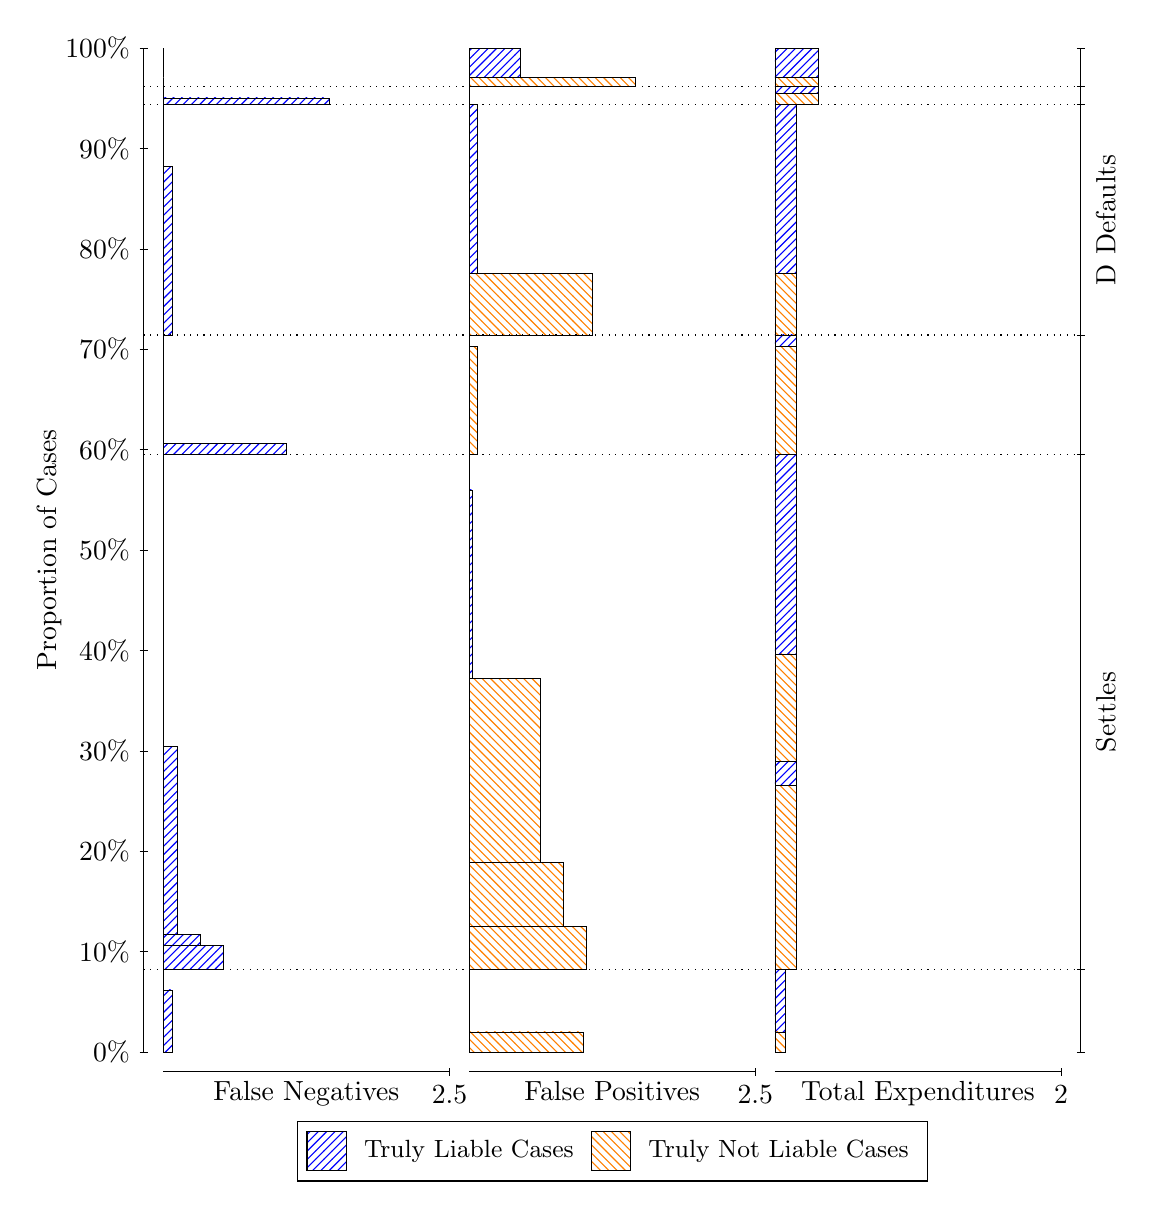
\begin{tikzpicture}
\draw[black, very thin] (1.5,1.75) -- (1.5,14.5);
\node[rotate=90, text=black, anchor=center] at (0.3, 8.125) {Proportion of Cases};
\draw[black, very thin] (1.45,1.75) -- (1.55,1.75);
\node[text=black, anchor=east] at (1.45, 1.75) {0\%};
\draw[black, very thin] (1.45,3.025) -- (1.55,3.025);
\node[text=black, anchor=east] at (1.45, 3.025) {10\%};
\draw[black, very thin] (1.45,4.3) -- (1.55,4.3);
\node[text=black, anchor=east] at (1.45, 4.3) {20\%};
\draw[black, very thin] (1.45,5.575) -- (1.55,5.575);
\node[text=black, anchor=east] at (1.45, 5.575) {30\%};
\draw[black, very thin] (1.45,6.85) -- (1.55,6.85);
\node[text=black, anchor=east] at (1.45, 6.85) {40\%};
\draw[black, very thin] (1.45,8.125) -- (1.55,8.125);
\node[text=black, anchor=east] at (1.45, 8.125) {50\%};
\draw[black, very thin] (1.45,9.4) -- (1.55,9.4);
\node[text=black, anchor=east] at (1.45, 9.4) {60\%};
\draw[black, very thin] (1.45,10.675) -- (1.55,10.675);
\node[text=black, anchor=east] at (1.45, 10.675) {70\%};
\draw[black, very thin] (1.45,11.95) -- (1.55,11.95);
\node[text=black, anchor=east] at (1.45, 11.95) {80\%};
\draw[black, very thin] (1.45,13.225) -- (1.55,13.225);
\node[text=black, anchor=east] at (1.45, 13.225) {90\%};
\draw[black, very thin] (1.45,14.5) -- (1.55,14.5);
\node[text=black, anchor=east] at (1.45, 14.5) {100\%};

\draw[black, very thin] (13.4,1.75) -- (13.4,14.5);
\draw[black, very thin] (13.35,1.75) -- (13.45,1.75);
\node[anchor=west] at (13.35, 1.75) {};
\draw[black, very thin] (13.35,2.7957) -- (13.45,2.7957);
\node[anchor=west] at (13.35, 2.7957) {};
\draw[black, very thin] (13.35,9.3367) -- (13.45,9.3367);
\node[anchor=west] at (13.35, 9.3367) {};
\draw[black, very thin] (13.35,10.856) -- (13.45,10.856);
\node[anchor=west] at (13.35, 10.856) {};
\draw[black, very thin] (13.35,13.782) -- (13.45,13.782);
\node[anchor=west] at (13.35, 13.782) {};
\draw[black, very thin] (13.35,14.017) -- (13.45,14.017);
\node[anchor=west] at (13.35, 14.017) {};
\draw[black, very thin] (13.35,14.5) -- (13.45,14.5);
\node[anchor=west] at (13.35, 14.5) {};

\draw[black, very thin, pattern color=blue, pattern=north east lines] (1.75,1.75) rectangle (1.859,2.5393);
\draw[black, very thin, pattern color=orange, pattern=north west lines] (1.75,2.5393) rectangle (1.75,2.7957);
\draw[black, very thin, pattern color=blue, pattern=north east lines] (1.75,2.7957) rectangle (2.513,3.1012);
\draw[black, very thin, pattern color=blue, pattern=north east lines] (1.75,3.1012) rectangle (2.2223,3.2427);
\draw[black, very thin, pattern color=blue, pattern=north east lines] (1.75,3.2427) rectangle (1.9317,5.6336);
\draw[black, very thin, pattern color=orange, pattern=north west lines] (1.75,5.6336) rectangle (1.75,9.3367);
\draw[black, very thin, pattern color=blue, pattern=north east lines] (1.75,9.3367) rectangle (3.3123,9.4788);
\draw[black, very thin, pattern color=orange, pattern=north west lines] (1.75,9.4788) rectangle (1.75,10.856);
\draw[black, very thin, pattern color=blue, pattern=north east lines] (1.75,10.856) rectangle (1.859,13);
\draw[black, very thin, pattern color=orange, pattern=north west lines] (1.75,13) rectangle (1.75,13.782);
\draw[black, very thin, pattern color=blue, pattern=north east lines] (1.75,13.782) rectangle (3.8573,13.868);
\draw[black, very thin, pattern color=orange, pattern=north west lines] (1.75,13.868) rectangle (1.75,14.017);
\draw[black, very thin, pattern color=orange, pattern=north west lines] (1.75,14.017) rectangle (1.75,14.124);
\draw[black, very thin, pattern color=blue, pattern=north east lines] (1.75,14.124) rectangle (1.75,14.5);
\draw[black, very thin, pattern color=orange, pattern=north west lines] (5.6333,1.75) rectangle (7.0867,2.0064);
\draw[black, very thin, pattern color=blue, pattern=north east lines] (5.6333,2.0064) rectangle (5.6333,2.7957);
\draw[black, very thin, pattern color=orange, pattern=north west lines] (5.6333,2.7957) rectangle (7.123,3.3477);
\draw[black, very thin, pattern color=orange, pattern=north west lines] (5.6333,3.3477) rectangle (6.8323,4.1579);
\draw[black, very thin, pattern color=orange, pattern=north west lines] (5.6333,4.1579) rectangle (6.5417,6.4989);
\draw[black, very thin, pattern color=blue, pattern=north east lines] (5.6333,6.4989) rectangle (5.6697,8.8897);
\draw[black, very thin, pattern color=blue, pattern=north east lines] (5.6333,8.8897) rectangle (5.6333,9.3367);
\draw[black, very thin, pattern color=orange, pattern=north west lines] (5.6333,9.3367) rectangle (5.7423,10.714);
\draw[black, very thin, pattern color=blue, pattern=north east lines] (5.6333,10.714) rectangle (5.6333,10.856);
\draw[black, very thin, pattern color=orange, pattern=north west lines] (5.6333,10.856) rectangle (7.1957,11.638);
\draw[black, very thin, pattern color=blue, pattern=north east lines] (5.6333,11.638) rectangle (5.7423,13.782);
\draw[black, very thin, pattern color=orange, pattern=north west lines] (5.6333,13.782) rectangle (5.6333,13.931);
\draw[black, very thin, pattern color=blue, pattern=north east lines] (5.6333,13.931) rectangle (5.6333,14.017);
\draw[black, very thin, pattern color=orange, pattern=north west lines] (5.6333,14.017) rectangle (7.7407,14.124);
\draw[black, very thin, pattern color=blue, pattern=north east lines] (5.6333,14.124) rectangle (6.2873,14.5);
\draw[black, very thin, pattern color=orange, pattern=north west lines] (9.5167,1.75) rectangle (9.6529,2.0064);
\draw[black, very thin, pattern color=blue, pattern=north east lines] (9.5167,2.0064) rectangle (9.6529,2.7957);
\draw[black, very thin, pattern color=orange, pattern=north west lines] (9.5167,2.7957) rectangle (9.7892,5.1366);
\draw[black, very thin, pattern color=blue, pattern=north east lines] (9.5167,5.1366) rectangle (9.7892,5.4421);
\draw[black, very thin, pattern color=orange, pattern=north west lines] (9.5167,5.4421) rectangle (9.7892,6.8043);
\draw[black, very thin, pattern color=blue, pattern=north east lines] (9.5167,6.8043) rectangle (9.7892,9.3367);
\draw[black, very thin, pattern color=orange, pattern=north west lines] (9.5167,9.3367) rectangle (9.7892,10.714);
\draw[black, very thin, pattern color=blue, pattern=north east lines] (9.5167,10.714) rectangle (9.7892,10.856);
\draw[black, very thin, pattern color=orange, pattern=north west lines] (9.5167,10.856) rectangle (9.7892,11.638);
\draw[black, very thin, pattern color=blue, pattern=north east lines] (9.5167,11.638) rectangle (9.7892,13.782);
\draw[black, very thin, pattern color=orange, pattern=north west lines] (9.5167,13.782) rectangle (10.062,13.931);
\draw[black, very thin, pattern color=blue, pattern=north east lines] (9.5167,13.931) rectangle (10.062,14.017);
\draw[black, very thin, pattern color=orange, pattern=north west lines] (9.5167,14.017) rectangle (10.062,14.124);
\draw[black, very thin, pattern color=blue, pattern=north east lines] (9.5167,14.124) rectangle (10.062,14.5);
\draw[black, dotted] (1.5,2.7957) -- (13.4,2.7957);
\draw[black, dotted] (1.5,9.3367) -- (13.4,9.3367);
\draw[black, dotted] (1.5,10.856) -- (13.4,10.856);
\draw[black, dotted] (1.5,13.782) -- (13.4,13.782);
\draw[black, dotted] (1.5,14.017) -- (13.4,14.017);
\draw[black, very thin] (1.75,1.5) -- (5.3833,1.5);
\node[text=black, anchor=north] at (3.5667, 1.5) {False Negatives};
\draw[black, very thin] (5.3833,1.45) -- (5.3833,1.55);
\node[text=black, anchor=north] at (5.3833, 1.45) {2.5};

\draw[black, very thin] (5.6333,1.5) -- (9.2667,1.5);
\node[text=black, anchor=north] at (7.45, 1.5) {False Positives};
\draw[black, very thin] (9.2667,1.45) -- (9.2667,1.55);
\node[text=black, anchor=north] at (9.2667, 1.45) {2.5};

\draw[black, very thin] (9.5167,1.5) -- (13.15,1.5);
\node[text=black, anchor=north] at (11.333, 1.5) {Total Expenditures};
\draw[black, very thin] (13.15,1.45) -- (13.15,1.55);
\node[text=black, anchor=north] at (13.15, 1.45) {2};


\node[text=black, centered, rotate=90] at (13.72, 6.0662) {Settles};

\node[text=black, centered, rotate=90] at (13.72, 12.319) {D Defaults};



\draw (7.449999999999999,1.5) node[draw=none] (baseCoordinate) {};
\begin{scope}[align=center]
        \matrix[scale=0.5, draw=black, below=0.5cm of baseCoordinate, nodes={draw}, column sep=0.1cm]{
            \node[rectangle, draw, minimum width=0.5cm, minimum height=0.5cm, pattern color=blue, pattern=north east lines] {}; &
            \node[draw=none, font=\small, text=black] (B) {Truly Liable Cases}; &
            \node[rectangle, draw, minimum width=0.5cm, minimum height=0.5cm, pattern color=orange, pattern=north west lines] {}; &
            \node[draw=none, font=\small, text=black] (B) {Truly Not Liable Cases}; \\
            };
\end{scope}

\end{tikzpicture}
\end{document}